% To compile single chapters put a % symbol in front of "\comment" and "}%end of comment" below 
%    and take off the % symbol from "\end{document" at the bottom line. Undo before compiling
%    the complete thesis
%%Note: You can only use \section command, you are not allowed, per TTU Graduate School, use
%%\subsection command for ghigher level subheadings. At most level 2 subheadings are allowed.

\chapter{Experiments and Results}
\label{Experiments and Results}

\section[Simulation Overview]{Testing Overview}

Two machine learning approaches are utilized in Chapter \ref{DASP Device Classification Chapter} to determine the performance and applicability of DASP originated features for URE characterization and classification.  A feature vector approach using LDA and k-NN learning algorithms was applied to the 1-D statistical feature vectors derived from DASP images, as described in Section \ref{Statistical Feature Extraction}, while a CNN deep learning algorithm was applied directly to the DASP images to perform image recognition based learning. Figure \ref{fig:dasp_lda_knn_process_flow} provides a detailed diagram of the DASP feature vector processing flow from URE signal capture to the LDA and k-NN learning algorithms. 

\begin{figure}[tb]
	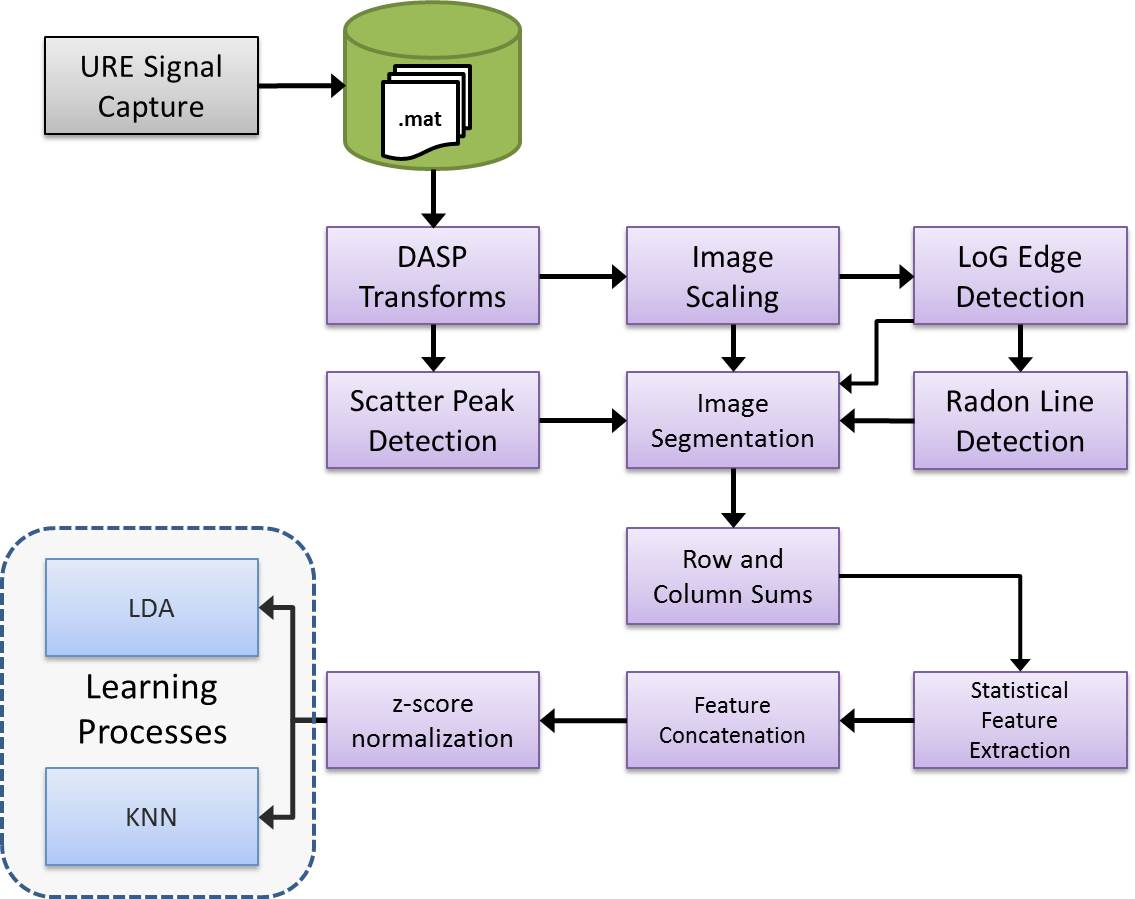
\includegraphics[width=\textwidth]{./misc_graphics/dasp_lda_knn_process_flow.jpg}
	\centering
	\caption{Flow diagram of the DASP processing flow from URE signal capture through the LDA and k-NN learning process.}
	\label{fig:dasp_lda_knn_process_flow}
\end{figure}
 
Figure \ref{fig:dasp_lda_knn_process_flow} outlines the DASP processing flow to generate feature vectors for LDA and k-NN testing and training.   All URE signal captures were initially processed through the DASP transforms with up to four images extracted from each DASP transform, the raw scaled image, the scatter peak detector image, the LoG edge detector image, and the radon line detector image.  Statistical feature vectors were then extracted from the DASP images by first segmenting the image and then performing row and column summing to obtain statistical sample vectors.  The statistical measurements were then concatenated in to a 1-D feature vector per sample and normalized by their z-score across all samples.  The normalized feature vectors were evaluated through the LDA and k-NN learning processes.

Figure \ref{fig:dasp_cnn_process_flow} provides an overview of the DASP processing flow for the CNN learning process.  Instead of image segmentation and feature vector extraction, the CNN learner only requires an image input for learning.  Similar to the feature vector processing flow, the CNN process generates up to four images for each DASP transform, the raw scaled image, the scatter peak detector image, the LoG edge detector image, and the radon line detector image.  The resulting DASP images were saved as individual Tag Image File Format (TIFF) files for cataloging, labeling, training, and testing with the CNN learner.

\begin{figure}[tb]
	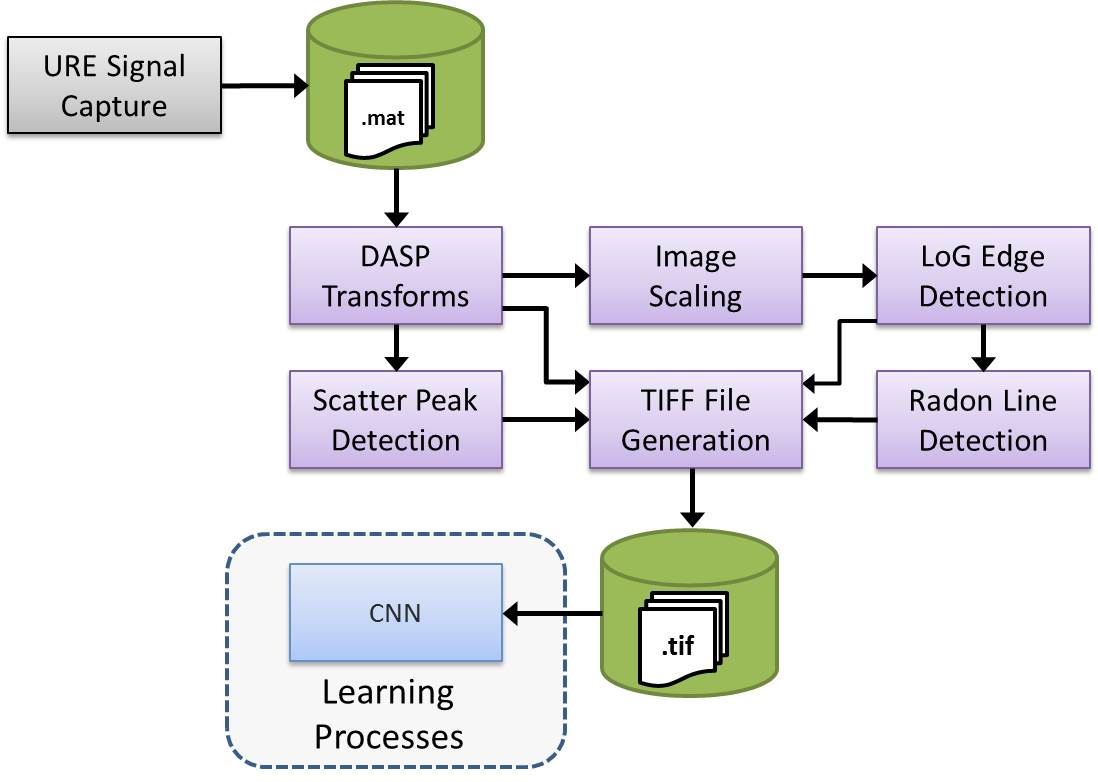
\includegraphics[width=\textwidth]{./misc_graphics/dasp_cnn_process_flow.jpg}
	\centering
	\caption{Flow diagram of the DASP processing flow from URE signal capture through the CNN learning process.}
	\label{fig:dasp_cnn_process_flow}
\end{figure}

\section[DASP Processes and Transforms]{DASP Processes and Transforms}

Because no \emph{a priori} knowledge of the test devices' URE characteristics were taken in to account in the DASP evaluation process, the DASP algorithms, transforms, and parameter settings were selected heuristically to include as much of the URE spectrum that could be reasonably achieved given a $2$MS/s collection system and a one second capture time per device sample.  Table \ref{tab:dasp_config_parameters} provides a listing of the DASP algorithms and transforms used in the feature and image generation processes, along with their respective parameter settings.  All DASP algorithms were evaluated, including the SCAP auto-covariance vector, $\bf{S}_F$, while it should also be noted that not all combinations of DASP algorithms and image processing transforms were utilized.  In addition, the SCAP auto-covariance vector was not utilized by the CNN learner because it does not result in a 2-D image. 

\begin{table}[tb]
	\caption{Table of all DASP algorithms and image transforms used for image generation and feature extraction.}
	\centering
		\begin{tabular}{cc|c}
		\hline
		DASP Algorithm & Image Transform & Configuration Parameters\\
		\hline
    CMASP & Array & $f_c = 10000$\\
		CMASP & Edge Array & $Bc = 9500$ \\
		CMASP & Radon Array & $f_m = 1000$ \\
		& & $B_m = 950$ \\
		\hline
		FASP & Array & $N = 1000$ \\
		\hline
		HASP-F & Array & $f_c = 1000$ \\
		HASP-F & Edge Array & $B = 1990$ \\
		HASP-F & Radon Array & \\
		\hline
		HASP-D & Array & $f_c = 1000$ \\
		& & $B = 1990$ \\
		\hline
		MASP (Low) & Array & $N = 10000$\\
		MASP (Low) & Edge Array & $p = 0.02$ \\
		MASP (Low) & Radon Array & \\
		MASP (Low) & Scatter Plot &\\
		\hline
		MASP (High) & Array & $N = 1000$ \\
		MASP (High) & Edge Array & $p = 0.02$ \\
		MASP (High) & Radon Array & \\
		MASP (High) & Scatter Plot & \\	
		\hline
		SCAP & Array & $f_c = 1000$ \\
		SCAP & Cross-Covariance Vector & $B = 1990$ \\
    \hline
		\end{tabular}
	\label{tab:dasp_config_parameters}
\end{table}

Table \ref{tab:dasp_config_parameters} provides the configuration parameters for each DASP algorithm, based upon their specific input requirements.  Two sets of MASP images were generated with different settings to characterize low and high frequency modulations, with the higher frequency MASP algorithm trading off modulation frequency resolution.  The Edge and Radon Arrays were not applied to the FASP, HASP-D, and SCAP images because the additional benefit was not obvious given the multitude of curved lines present in the HASP-D and SCAP images and the large number of vertical lines in a typical FASP image.

\section[Statistical Feature Extraction]{Statistical Feature Extraction}

Statistical features were extracted from the whole and $3 \times 3$ segmented DASP images in Table \ref{tab:dasp_config_parameters} using the whole image, the summed row vector, and the summed column vector.  The extracted features for each image segment were concatenated in to a single feature vector 
\begin{equation}
	\textit{\textbf{X}}_s= [\sigma^{2}_{\omega},  \gamma_{\omega},  \kappa_{\omega}, \sigma^{2}_{\rho},  \gamma_{\rho},  \kappa_{\rho}, \sigma^{2}_{\gamma},  \gamma_{\gamma},  \kappa_{\gamma}]
	\label{eq:featureeq}
\end{equation}
where $\omega$ are the whole segment features, $\rho$ are summed row features, and $\gamma$ are summed column features, resulting in $9$ features for each of the DASP image segments.  The SCAP auto-covariance vector only provides a single vector for feature extraction and therefore only yielded three features, $[\sigma^{2},  \gamma,  \kappa]$.  Finally, the z-score for each feature was calculated across all data sets resulting in a normalized feature set that was utilized for subsequent training and classification analysis.  The image segment feature vectors, $\textit{\textbf{X}}_s$, were then concatenated to form a full feature vector
\begin{equation}
	\textit{\textbf{X}}= [\textit{\textbf{X}}_1, \textit{\textbf{X}}_2, \ldots, \textit{\textbf{X}}_9, \textit{\textbf{X}}_{10}]
	\label{eq:featureeq_cat}
\end{equation}
for each DASP image, where $\textit{\textbf{X}}_1$ is the top image segment and $\textit{\textbf{X}}_2$ through $\textit{\textbf{X}}_{10}$ are the $9$ image segments comprised of the $3 \times 3$ grid segmentation.  The concatenation of the image segment feature vectors resulted in a total of $9 \times 10 = 90$ features per DASP image, except for the SCAP auto-covariance feature vector which only returned three features.

\section[DASP Image Store]{DASP Image Store}

The MATLAB\textsuperscript \textregistered ~~Convolutional Neural Network implementation, including supporting tools such as the \textit{imageDataStore} command, was designed to seamlessly catalog, label, train, and test on image files.  To simplify the CNN learning process, each DASP image was saved as a \textit{.tif} file using the process in Algorithm \ref{alg:tiffimalg}.  The TIFF image generation algorithm is identical to the image scaling algorithm, Algorithm \ref{alg:imscalealg}, with the addition of the $16$bit scaling, image resizing, and file saving steps.  Each TIFF file was stored in its own directory structure within a labeled folder for class indexing.

\begin{algorithm}
	\caption{TIFF Image Generation Algorithm} \label{alg:tiffimalg}
	\scriptsize
	\begin{algorithmic}[1]
		\Require~~
		\Statex $\mathbf{I}$ - Input Image
		\Statex $\mathbf{I_b}$ - Background Image
		\Ensure~~
		\Statex $\mathbf{I_s}$ - Saved TIFF Image
		\Statex
		\State $\mathbf{I_s} \gets \mathbf{I} - \mathbf{I_b}$ 
		\State $\mathbf{I_s} \leq 0 \gets 0$
		\State $\mathbf{I_s}  \gets $ STANDARD DEVIATION FILTER of $\mathbf{I_s}$
		\State $\mathbf{I_s} \gets \log{\mathbf{I_s}}$
		\State $\mathbf{I_s} \gets 2^{16} \times \frac{\mathbf{I_s} - \min{\mathbf{I_s}}}{\max{\mathbf{I_s}} - \min{\mathbf{I_s}}}$
		\State RESIZE $\mathbf{I_s}$ to $500 \times 500$
		\State SAVE $\mathbf{I_s}$ as $16$bit TIFF Image file
	\end{algorithmic}
\end{algorithm}
